\section{Das dreieinige Gehirn}\label{sec:das-dreieinige-gehirn}
Körpersprachliche Verhaltensmuster können zwischen Menschen kultur- und gesellschaftsübergreifend ausgedrückt und verstanden werden.

Eine erklärung für diese Gemeinsamkeiten im Verhalten der Menschen zeigt das Modell des dreieinigen Gehirns
vom US-amerikanischen Hirnforscher Paul D. MacLean.

Dieses Modell gliedert das Gehirn in drei Subsysteme auf, welche in den nachfolgenden Abschnitten genauer beschrieben werden:
Das protoreptilische, das paläomammalische und das neomammalische Gehirn.

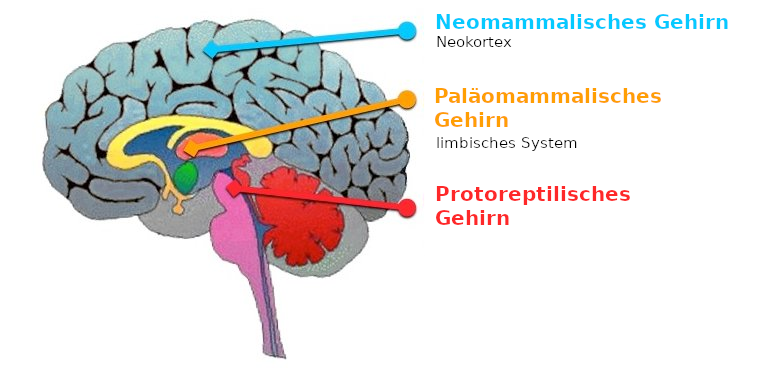
\includegraphics[width=\textwidth]{images/brain}

\subsection{Das protoreptilische Gehirn}\label{subsec:das-protoreptilische-gehirn}

Dieser Teil des Gehirns, auch Reptil- oder Stammhirn genannt, ist für alle primitivsten Funktionen im Körper zuständig.
Beispielsweise wird hier die Atmung, der Schlaf, das Erwachen usw.\ gesteuert.

\subsection{Das paläomammalische Gehirn}\label{subsec:das-palaomammalische-gehirn}
Andere Namen für diesen Teil des Gehirns sind auch das \textit{limbische System} oder emotionales Gehirn.
Dieser Hirnteil befindet sich im Zentrum des zentralen Nervensystems, direkt über dem protoreptilischen Gehirn.

Dieser Teil des gehirns, ist die Zentrale welche unsere tief verankerten Reaktionen auf behagliche und unbehagliche
Situationen in Form nonverbaler Kommunikation ausdrückt.

\subsection{Das neomammalische Gehirn}\label{subsec:das-neomammalische-gehirn}
Der auch als Neokortex bekannte Teil des Gehirns ist unter den drei Hirnteilen der jüngste.
Rationelles Denken findet hier statt.
In Bezug auf nonverbale Kommunikation ist relevant zu wissen, dass dieser Teil des Gehirns derjenige ist,
welcher für die Aktive unterdrückung oder beeinflussung nonverbaler Kommunikation ist.
Möchten wir beispielsweise unser Lachen unterdrücken, ist dies der Teil des Gehirns, welcher diese Entscheidung und Steuerung veranlasst.